%\chapter{In-text Elements}
%
%\section{Theorems}\index{Theorems}
%
%This is an example of theorems.
%
%\subsection{Several equations}\index{Theorems!Several Equations}
%This is a theorem consisting of several equations.
%
%\begin{theorem}[Name of the theorem]
%In $E=\mathbb{R}^n$ all norms are equivalent. It has the properties:
%\begin{align}
%& \big| ||\mathbf{x}|| - ||\mathbf{y}|| \big|\leq || \mathbf{x}- \mathbf{y}||\\
%&  ||\sum_{i=1}^n\mathbf{x}_i||\leq \sum_{i=1}^n||\mathbf{x}_i||\quad\text{where $n$ is a finite integer}
%\end{align}
%\end{theorem}
%
%\subsection{Single Line}\index{Theorems!Single Line}
%This is a theorem consisting of just one line.
%
%\begin{theorem}
%A set $\mathcal{D}(G)$ in dense in $L^2(G)$, $|\cdot|_0$. 
%\end{theorem}
%
%%------------------------------------------------
%
%\section{Definitions}\index{Definitions}
%
%This is an example of a definition. A definition could be mathematical or it could define a concept.
%
%\begin{definition}[Definition name]
%Given a vector space $E$, a norm on $E$ is an application, denoted $||\cdot||$, $E$ in $\mathbb{R}^+=[0,+\infty[$ such that:
%\begin{align}
%& ||\mathbf{x}||=0\ \Rightarrow\ \mathbf{x}=\mathbf{0}\\
%& ||\lambda \mathbf{x}||=|\lambda|\cdot ||\mathbf{x}||\\
%& ||\mathbf{x}+\mathbf{y}||\leq ||\mathbf{x}||+||\mathbf{y}||
%\end{align}
%\end{definition}
%
%%------------------------------------------------
%
%\section{Notations}\index{Notations}
%
%\begin{notation}
%Given an open subset $G$ of $\mathbb{R}^n$, the set of functions $\varphi$ are:
%\begin{enumerate}
%\item Bounded support $G$;
%\item Infinitely differentiable;
%\end{enumerate}
%a vector space is denoted by $\mathcal{D}(G)$. 
%\end{notation}
%
%%------------------------------------------------
%
%\section{Remarks}\index{Remarks}
%
%This is an example of a remark.
%
%\begin{remark}
%The concepts presented here are now in conventional employment in mathematics. Vector spaces are taken over the field $\mathbb{K}=\mathbb{R}$, however, established properties are easily extended to $\mathbb{K}=\mathbb{C}$.
%\end{remark}
%
%%------------------------------------------------
%
%\section{Corollaries}\index{Corollaries}
%
%This is an example of a corollary.
%
%\begin{corollary}[Corollary name]
%The concepts presented here are now in conventional employment in mathematics. Vector spaces are taken over the field $\mathbb{K}=\mathbb{R}$, however, established properties are easily extended to $\mathbb{K}=\mathbb{C}$.
%\end{corollary}
%
%%------------------------------------------------
%
%\section{Propositions}\index{Propositions}
%
%This is an example of propositions.
%
%\subsection{Several equations}\index{Propositions!Several Equations}
%
%\begin{proposition}[Proposition name]
%It has the properties:
%\begin{align}
%& \big| ||\mathbf{x}|| - ||\mathbf{y}|| \big|\leq || \mathbf{x}- \mathbf{y}||\\
%&  ||\sum_{i=1}^n\mathbf{x}_i||\leq \sum_{i=1}^n||\mathbf{x}_i||\quad\text{where $n$ is a finite integer}
%\end{align}
%\end{proposition}
%
%\subsection{Single Line}\index{Propositions!Single Line}
%
%\begin{proposition} 
%Let $f,g\in L^2(G)$; if $\forall \varphi\in\mathcal{D}(G)$, $(f,\varphi)_0=(g,\varphi)_0$ then $f = g$. 
%\end{proposition}
%
%%------------------------------------------------
%
%\section{Examples}\index{Examples}
%
%This is an example of examples.
%
%\subsection{Equation and Text}\index{Examples!Equation and Text}
%
%\begin{example}
%Let $G=\{x\in\mathbb{R}^2:|x|<3\}$ and denoted by: $x^0=(1,1)$; consider the function:
%\begin{equation}
%f(x)=\left\{\begin{aligned} & \mathrm{e}^{|x|} & & \text{si $|x-x^0|\leq 1/2$}\\
%& 0 & & \text{si $|x-x^0|> 1/2$}\end{aligned}\right.
%\end{equation}
%The function $f$ has bounded support, we can take $A=\{x\in\mathbb{R}^2:|x-x^0|\leq 1/2+\epsilon\}$ for all $\epsilon\in\intoo{0}{5/2-\sqrt{2}}$.
%\end{example}
%
%\subsection{Paragraph of Text}\index{Examples!Paragraph of Text}
%
%\begin{example}[Example name]
%\lipsum[2]
%\end{example}
%
%%------------------------------------------------
%
%\section{Exercises}\index{Exercises}
%
%This is an example of an exercise.
%
%\begin{exercise}
%This is a good place to ask a question to test learning progress or further cement ideas into students' minds.
%\end{exercise}
%
%%------------------------------------------------
%
%\section{Problems}\index{Problems}
%
%\begin{problem}
%What is the average airspeed velocity of an unladen swallow?
%\end{problem}
%
%%------------------------------------------------
%
%\section{Vocabulary}\index{Vocabulary}
%
%Define a word to improve a students' vocabulary.
%
%\begin{vocabulary}[Word]
%Definition of word.
%\end{vocabulary}


\chapter{Connections}

\section{Cipher suit}
A cipher suite is a set of algorithms that help secure a network connection that uses Transport Layer Security (TLS) or its now-deprecated predecessor Secure Socket Layer (SSL). The set of algorithms that cipher suites usually contain include: a key exchange algorithm, a bulk encryption algorithm, and a message authentication code (MAC) algorithm.\cite{ciphersuit-wiki}
\\
The key exchange algorithm is used to exchange a key between two devices. This key is used to encrypt and decrypt the messages being sent between two machines. The bulk encryption algorithm is used to encrypt the data being sent. The MAC algorithm provides data integrity checks to ensure that the data sent does not change in transit. In addition, cipher suites can include signatures and an authentication algorithm to help authenticate the server and or client.\cite{ciphersuit-wiki}
\\
After coordinating which cipher suite to use, the server and the client still has the ability to change the coordinated ciphers by using the ChangeCipherSpec protocol in the current handshake or in a new handshake.\cite{ciphersuit-wiki}


\subsection{TLS 1.0–1.2 handshake}

This client starts the process by sending a clientHello message to the server that includes the version of TLS being used and a list of cipher suites in the order of the client’s preference. In response, the server sends a serverHello message that includes the chosen cipher suite and the session ID. Next the server sends a digital certificate to verify its identity to the client. \textbf{The server may also request a client’s digital certification if needed}.\cite{ciphersuit-wiki}

\begin{figure}[!h]
\centering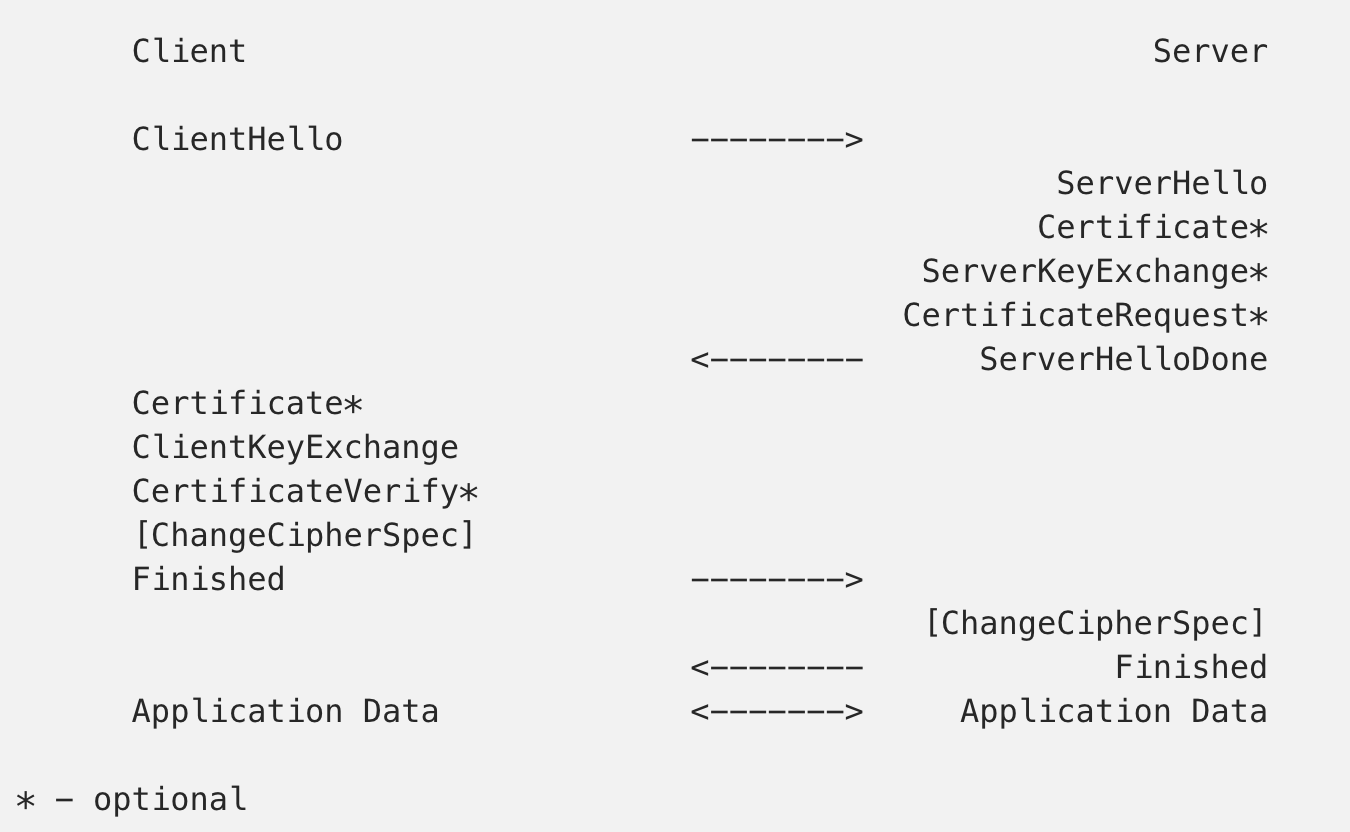
\includegraphics[scale=0.6]{TLS-Handshake}
\caption{TLS Handshake Protocol \cite{TLS-meduim}}
\label{fig:TLS_Proto} % Unique label used for referencing the figure in-text
\end{figure}


If the client and server are not using pre-shared keys, the client then sends an encrypted message to the server that enables the client and the server to be able to compute which secret key will be used during exchanges.\cite{ciphersuit-wiki}
\\
After successfully verifying the authentication of the server and, if needed, exchanging the secret key, the client sends a finished message to signal that it is done with the handshake process. After receiving this message, the server sends a finished message that confirms that the handshake is complete. Now the client and the server are in agreement on which cipher suite to use to communicate with each other.\cite{ciphersuit-wiki}


\begin{figure}[!h]
\centering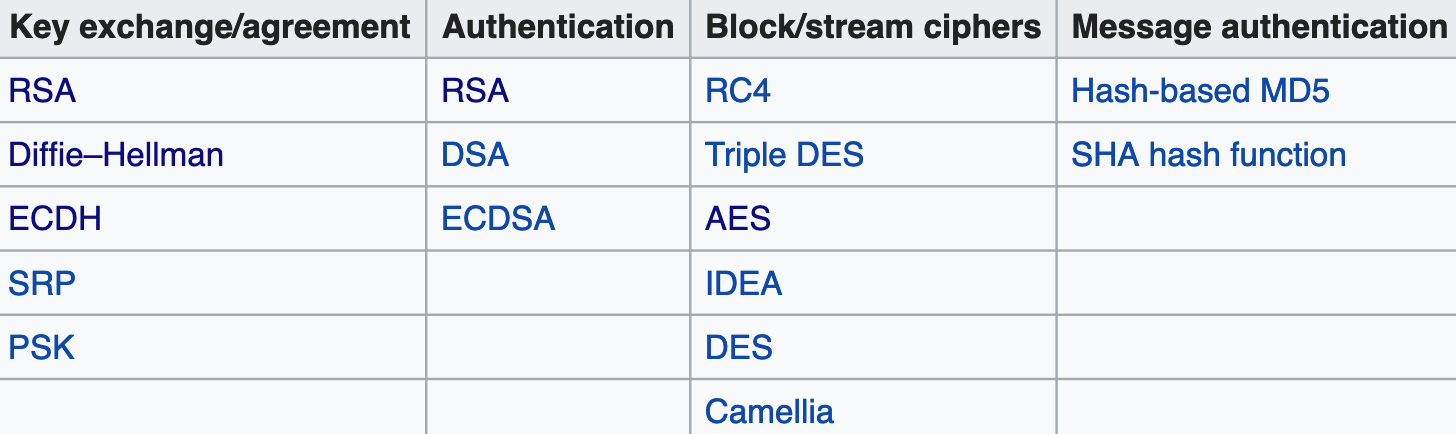
\includegraphics[scale=0.6]{TLSv1-12_algs}
\caption{Algorithms supported in TLS 1.0–1.2 cipher suites \cite{ciphersuit-wiki}}
\label{fig:TLS_algs} % Unique label used for referencing the figure in-text
\end{figure}

\section{Connections}

Connections between two Tor relays, or between a client and a relay, use TLS/SSLv3 for link authentication and encryption. All implementations MUST support the SSLv3 ciphersuite\\ "TLS\_DHE\_RSA\_WITH\_AES\_128\_CBC\_SHA" if it is available. They SHOULD support better ciphersuites if available.
\\

   There are three ways to perform TLS handshakes with a Tor server. 
   
   \begin{enumerate}
   	\item \textbf{certificates-up-front}: Both the initiator and responder send a two-certificate chain as part of their initial handshake.  (This is supported in all Tor versions.)
   	\item \textbf{renegotiation}: The responder provides a single certificate, and the initiator immediately performs a TLS renegotiation. (This is supported in Tor 0.2.0.21 and later.)
   	\item \textbf{in-protocol}: the initial TLS negotiation completes, and the parties bootstrap themselves to mutual authentication via use of the Tor protocol without further TLS handshaking. (This is supported in 0.2.3.6-alpha and later.)
   \end{enumerate}
   
  Each of these options provides a way for the parties to learn it is
   available: a client does not need to know the version of the Tor
   server in order to connect to it properly.
  
  
  
  
  
  
  
  
  
  
  